\chapter{Dataset}\label{chap:dataset}
In the following chapter the case studies considered in this thesis are detailed, specifically the datasets used and the preprocessing that later leads to the input of the proposed model.

\section{Video files}
The study case consists in analyzing high speed video data from GMAW processes, namely globular and spray transfer. The videos are raw \texttt{.cine} files which can be inspected using the \textit{Phantom Camera Control} (PCC) software. Since the processes are characterized by their transfer mode, one video for each is used. In tables \ref{table:glob_params} and \ref{table:spray_params} the parameters of each video are shown. 

After inspecting the metadata of the videos in PCC, they are read in \texttt{python} using the \texttt{pycine} library\footnote{\url{https://github.com/OTTOMATIC-IO/pycine}}. Then, each video is stored into an \texttt{.npz} file. In figures \ref{fig:glob_samples} and \ref{fig:spray_samples} frames of each transfer mode can be seen, particularly the main characteristic of larger droplets in globular and smaller droplets in spray\footnote{Similar videos found at \url{https://sites.ualberta.ca/~ccwj/videos/pages/Intro\%20High\%20Speed/}}.

Notice that later, to calculate physical properties of the process, there has to be a relationship between the pixels and real distance. This can be done using the wire's diameter, since that is a fixed length that is always visible in the image. Using that relationship, the pixel to distance conversion is

\begin{align}
    \text{Wire's diameter} &= 0.045\;in = 1.143\;mm = 26\;px \nonumber\\
    \xrightarrow{}1\;px &= 0.0439615\;mm =4.39615\cdot 10^{-5}\;m
    \label{eq:px_to_mm}
\end{align}

\begin{table}
\centering
\caption[Globular transfer video parameters]{Globular transfer video parameters.}
\label{table:glob_params}
\begin{tabular}{|l|l|lll}
\cline{1-2} \cline{4-5}
Electrode       & $ER70S-6$             & \multicolumn{1}{l|}{} & \multicolumn{1}{l|}{Shielding gas}     & \multicolumn{1}{l|}{$85\%$ $Ar$, $15\%$ $CO_2$} \\ \cline{1-2} \cline{4-5} 
Size            & $0.045''$ ($1.2$ $mm$)     & \multicolumn{1}{l|}{} & \multicolumn{1}{l|}{Number of frames}  & \multicolumn{1}{l|}{$9947$}              \\ \cline{1-2} \cline{4-5} 
Wire feed speed & $175$ $ipm$ ($4.4$ $m/min$) & \multicolumn{1}{l|}{} & \multicolumn{1}{l|}{Resolution}        & \multicolumn{1}{l|}{$352 \times 296$}           \\ \cline{1-2} \cline{4-5} 
Voltage         & $33$ $V$                 & \multicolumn{1}{l|}{} & \multicolumn{1}{l|}{Frame rate} & \multicolumn{1}{l|}{$3000\;Hz$}              \\ \cline{1-2} \cline{4-5} 
Travel speed    & $20$ $ipm$ ($0.5$ $m/min$)  & \multicolumn{1}{l|}{} & \multicolumn{1}{l|}{Period}            & \multicolumn{1}{l|}{$333.3$ $\mu s$}           \\ \cline{1-2} \cline{4-5} 
CTWD & $0.7''$ ($18$ $mm$) &\multicolumn{1}{l|}{} & \multicolumn{1}{l|}{File size}            & \multicolumn{1}{l|}{$2.01$ $Gb$}  \\ \cline{1-2}\cline{4-5} 
\end{tabular}
\end{table}

\begin{table}
\centering
\caption[Spray transfer video parameters]{Spray transfer video parameters.}
\label{table:spray_params}
\begin{tabular}{|l|l|lll}
\cline{1-2} \cline{4-5}
Electrode       & $ER70S-6$             & \multicolumn{1}{l|}{} & \multicolumn{1}{l|}{Shielding gas}     & \multicolumn{1}{l|}{$85\%$ $Ar$, $15\%$ $CO_2$} \\ \cline{1-2} \cline{4-5} 
Size            & $0.045''$ ($1.2$ $mm$)     & \multicolumn{1}{l|}{} & \multicolumn{1}{l|}{Number of frames}  & \multicolumn{1}{l|}{$6691$}              \\ \cline{1-2} \cline{4-5} 
Wire feed speed & $400$ $ipm$ ($10$ $m/min$) & \multicolumn{1}{l|}{} & \multicolumn{1}{l|}{Resolution}        & \multicolumn{1}{l|}{$352 \times 352$}           \\ \cline{1-2} \cline{4-5} 
Voltage         & $35$ $V$                 & \multicolumn{1}{l|}{} & \multicolumn{1}{l|}{Frame rate} & \multicolumn{1}{l|}{$3000\;Hz$}              \\ \cline{1-2} \cline{4-5} 
Travel speed    & $20$ $ipm$ ($0.5$ $m/min$)  & \multicolumn{1}{l|}{} & \multicolumn{1}{l|}{Period}            & \multicolumn{1}{l|}{$333.3$ $\mu s$}           \\ \cline{1-2} \cline{4-5} 
CTWD & $0.7''$ ($18$ $mm$) &\multicolumn{1}{l|}{} & \multicolumn{1}{l|}{File size}            & \multicolumn{1}{l|}{$1.61$ $Gb$}  \\ \cline{1-2}\cline{4-5} 
\end{tabular}
\end{table}




\begin{figure}
    \centering
    \begin{subfigure}[b]{0.3\textwidth}
        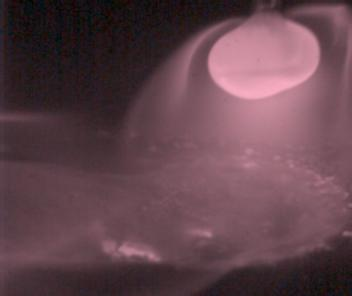
\includegraphics[width=\textwidth]{Images/Dataset/glob_sample_0.jpg}
        \caption{}
    \end{subfigure}
\hfill
    \begin{subfigure}[b]{0.3\textwidth}
        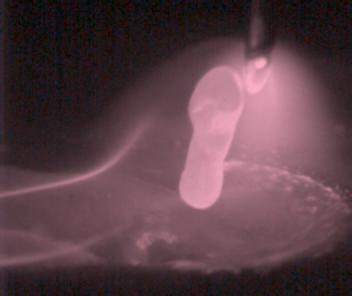
\includegraphics[width=\textwidth]{Images/Dataset/glob_sample_749.jpg}
        \caption{}
        \label{fig:glob_sample_irregular}
    \end{subfigure}
\hfill
    \begin{subfigure}[b]{0.3\textwidth}
        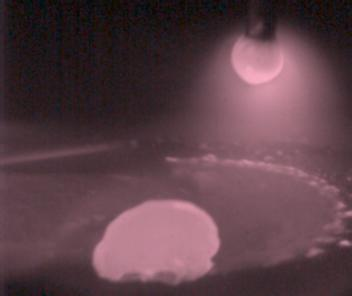
\includegraphics[width=\textwidth]{Images/Dataset/glob_sample_1506.jpg}
        \caption{}
    \end{subfigure}

    \caption[Globular transfer mode frames]{Globular transfer mode frames.}
    \label{fig:glob_samples}
\end{figure}

\begin{figure}[htbp]
    \centering
    \begin{subfigure}[b]{0.3\textwidth}
        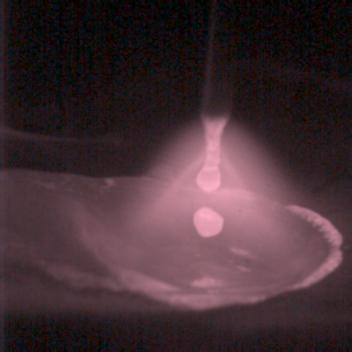
\includegraphics[width=\linewidth]{Images/Dataset/spray_sample_0.jpg}
        \caption{}
    \end{subfigure}
\hfill
    \begin{subfigure}[b]{0.3\textwidth}
        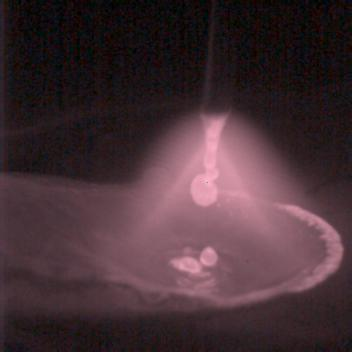
\includegraphics[width=\linewidth]{Images/Dataset/spray_sample_77.jpg}
        \caption{}
    \end{subfigure}
\hfill
    \begin{subfigure}[b]{0.3\textwidth}
        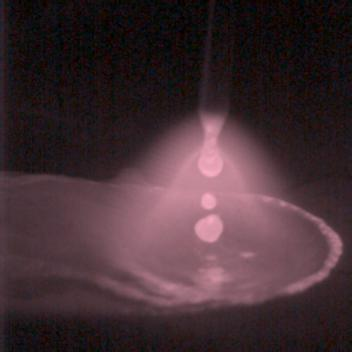
\includegraphics[width=\linewidth]{Images/Dataset/spray_sample_484.jpg}
        \caption{}
    \end{subfigure}

    \caption[Spray transfer mode frames]{Spray transfer mode frames.}
    \label{fig:spray_samples}
\end{figure}

\section{Labeling}
In order to train a supervised deep learning model, manual labels are made using the images as input. This is done using the LabelBox platform which allows to make such segmentation and then download the pairs of input image and corresponding mask. A number of 150 images were segmented for each transfer mode. Examples are shown in figures \ref{fig:glob_sample_masks} and \ref{fig:spray_sample_masks} for globular and transfer respectively.

\begin{figure}[htbp]
    \begin{subfigure}[b]{0.4\textwidth}
        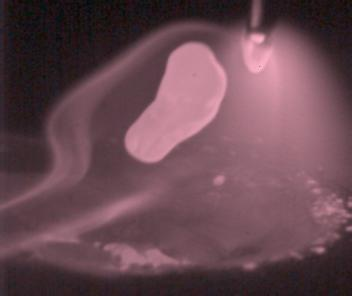
\includegraphics[width=\linewidth]{Images/Dataset/globular_image.jpg}
        \caption{Original frame}
    \end{subfigure}
\hfill
    \begin{subfigure}[b]{0.4\textwidth}
        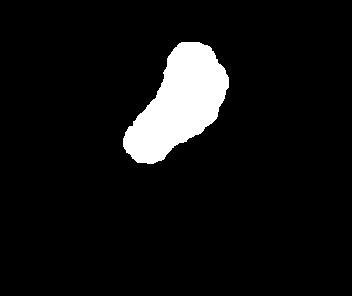
\includegraphics[width=\linewidth]{Images/Dataset/globular_mask.jpg}
        \caption{Manual segmentation mask}
    \end{subfigure}
    
    \caption[Examples of manually segmented frames for globular transfer]{Examples of manually segmented frames using LabelBox for globular transfer.}
    \label{fig:glob_sample_masks}
\end{figure}

\begin{figure}[htbp]
    \begin{subfigure}[b]{0.4\textwidth}
        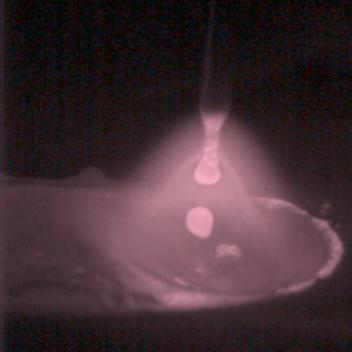
\includegraphics[width=\linewidth]{Images/Dataset/spray_image.jpg}
        \caption{Original frame}
    \end{subfigure}
\hfill
    \begin{subfigure}[b]{0.4\textwidth}
        
\includegraphics[width=\linewidth]{Images/Dataset/spray_mask.jpg}
        \caption{Manual segmentation mask}
    \end{subfigure}
    
    \caption[Examples of manually segmented frames for spray transfer]{Examples of manually segmented frames using LabelBox for spray transfer.}
    \label{fig:spray_sample_masks}
\end{figure}

The selection of the training images is not random, frames are chosen to have as much of the variety of the process as possible, that is the droplet formation, growth and release as well as some deviations such as irregular droplet shape (see figure \ref{fig:glob_sample_irregular}), horizontal droplet movement (as opposed to vertical), among others. Since most of the frames are from the growth process because it takes more time, it would be counterproductive to choose random frames because one would run into the risk of choosing most, if not all, images from the growth process, inadvertently ignoring the rest.

Notice that although the images have color, it is mostly a gradient from white to black through different intensities of magenta so the images are used as grayscale because the same information can be captured with a third of file size.

\section{Data augmentation}
A total of 150 images were labeled for each transfer mode. Since the number of images is low, data augmentation is used applying several alterations to the original images and labels. Each example is augmented such that it produces 5 different training examples. Therefore, the augmented dataset has 750 images for each transfer mode. In figure \ref{fig:augmented_sample}\footnote{Image \ref{fig:augmented_sample} has different colors compared to images in previous figures, this is due to the color map used when plotting the grayscale image in \texttt{matplotlib}. Nonetheless, pixel values are the same.} an example of an augmented input is shown and in table \ref{table:dataset_summary} a summary of the dataset information is shown.

Augmentations are made in \texttt{python} using the library \texttt{imgaug} and are listed as follows: 
\begin{itemize}
    \item Pixel dropout between $0\%$ and $5\%$, which means a probability is sampled uniformly such that $p \in [0, 0.05]$ for each augmented image so that every pixel has a probability $p$ of being turned to zero. In practice, every image will lose random pixels up to a maximum of $5\%$ of the whole image.
    \item Rotations between $-45^\circ$ and $45^\circ$.
    \item Elastic transformations with $\alpha \in [20, 50]$ and $\sigma\in [4,5]$ sampled uniformly from their respective intervals for each augmented image, where $\alpha$ is the strength of the distortion field. Higher values mean that pixels are moved further with respect to the distortion field's direction. $\sigma$ is the standard deviation of the Gaussian kernel used to smooth the distortion  
    fields. This gives the images a ripple effect.
    \item Additive Gaussian noise with mean $\mu=0$ and standard deviation $\sigma\in[0,15]$ sampled uniformly for each augmented image.
\end{itemize}

Notice in figure \ref{fig:augmented_sample} that the sampling of parameters within intervals for each image makes it so that some images are slightly changed while others are more heavily augmented. Also, the labels are only affected by the transformations that do not affect pixel intensity, such as elastic transformations and flips, and they are not affected by pixel dropping or Gaussian noise.
\begin{figure}
    \centering
    \import{Images/Dataset/augmented_sample/}{augmented_sample.pgf}
    \caption[Sample of an augmented image and mask]{Sample of an augmented image and respective mask (top left) using pixel dropout, rotation, elastic transformation and additive Gaussian noise. All the effects are applied simultaneously.}
    \label{fig:augmented_sample}
\end{figure}


\begin{table}
\centering
\caption{Dataset summary per transfer mode.}
\label{table:dataset_summary}
\begin{tabular}{|c|c|}
\hline
\begin{tabular}[c]{@{}c@{}}Complete\\ dataset\end{tabular} & \begin{tabular}[c]{@{}c@{}}9947 (globular)\\ 6691 (spray)\end{tabular}                       \\ \hline
\begin{tabular}[c]{@{}c@{}}Manually\\ segmented\end{tabular} & 150           \\ \hline
Augmented                                                    & 750           \\ \hline
Shape                                                      & \begin{tabular}[c]{@{}c@{}}$352\times 296$ (globular)\\ $352\times 352$ (spray)\end{tabular} \\ \hline
Channels|                                                    & 1 (grayscale) \\ \hline
\end{tabular}
\end{table}

